\documentclass[12pt]{article}
\usepackage[a4paper, margin=2cm]{geometry}
\usepackage[english]{babel} % To obtain English text with the blindtext package
\usepackage{blindtext}
\usepackage{graphicx} % Required for inserting images
\usepackage{array} % For extra column formatting
\usepackage{amsmath} %for equation environment
\usepackage{float}
\usepackage{parskip} % For gaps between para
\usepackage{setspace}
\usepackage{pdfpages}
\usepackage{abstract}
\usepackage[export]{adjustbox}
\usepackage{emptypage}
\usepackage{tocloft}
\usepackage[nottoc]{tocbibind}
\usepackage{url}


\cftsetindents{section}{0em}{2em}
\cftsetindents{subsection}{0em}{2em}

\renewcommand\cfttoctitlefont{\hfill\Large\bfseries}
\renewcommand\cftaftertoctitle{\hfill\mbox{}}

\graphicspath{ {./images/} }

\pagenumbering{arabic}


%%%%%%%%%%%%%%%%%%%%%%%%%%%%%%%%%%%


\title{PHYC20090 Exp.7 LCR Circuits}
\author{Joana Adao}
\date{\today}

\begin{document}

\begin{titlepage}
    \begin{center}

        \begin{figure}[ht]
            
\includegraphics[width=\textwidth]{UCDLogo.png}
        \end{figure}
        
        \begin{figure}
            \centerline{
\includegraphics[width=\paperwidth]{UCDBanner.png}}
        \end{figure}

        \vspace{4cm}

        {\Huge \bfseries PHYC20090 Electronics and Devices}\\
        \vspace{0.75cm}
        {\LARGE Experiment No.7 Sinusodial Response of the LCR Resonant Circuit }
        
        \vspace{1cm}
    
    {\Large \textbf{27 January 2025 }}

    \vspace{2cm}
    
    {\large \textbf{by Joana C.C. Adao (Student No. 23311051)}}\\
    \medskip
    {\large With Arminas A., Ananya L., Samuel S.}

    \end{center}
    
   \clearpage

\end{titlepage}

\setcounter{page}{1}
\tableofcontents

\newpage

\begin{abstract}
\addcontentsline{toc}{section}{Abstract}

The aim of this experiment was to



\end{abstract}


%%%%%%%%%%%%%%%%%%%%%%%%%%%%%%%%%%%


\section{Theory}

\subsection{LCR Circuits}
An LCR circuit is made up of inductors (L), capacitors (C), and resistors (R), usually connected in series.
Since all the components of the circuit are connected in series, equal amount of the current will flow through each element.
\cite{unacademy}

A circuit containing these components, L, C, and R, can act as themselves individually at certain frequencies
\cite{learnabout}, §1.2.1.
The LCR circuit can also magnify the voltages across the L, C, and R such that it is larger than the  circuit's input voltage (ie. AC, Alternating Current)
\cite{learnabout}.

\subsubsection{Inductance, Capacitance, Resistance}

Inductance, capacitance, and resistance make up the basic parameters that can affect circuits up to some degree
\cite{elecnotes}.

\textbf{Inductance} is a property of a conductor
\cite{britinductance}
and it's measured by its ability to store energy due to the magnetic field produced by the flow of current
\cite{elecnotes}
and the voltage that is induced by the current's rate of change
\cite{britinductance}.
With AC (Alternating Current), the magnetic field produced fluctuates with the time-varying properties of AC power sources
\cite{elecnotes,britinductance}.

The voltage is proportional to the rate of change of the current and this factor of proportionality is known as the inductance
\cite{britinductance}.
Coils of wire are most commonly used as the inductors in circuits as they amplify \cite{elecnotes} the efficiency at which the magnetic field induces
the voltage and current in the circuit. By coiling wire (solenoid) the magnetic field is concentrated and magnified at its centre, shown in Figure \ref{fig:solenoid}.

\begin{figure}[h]
    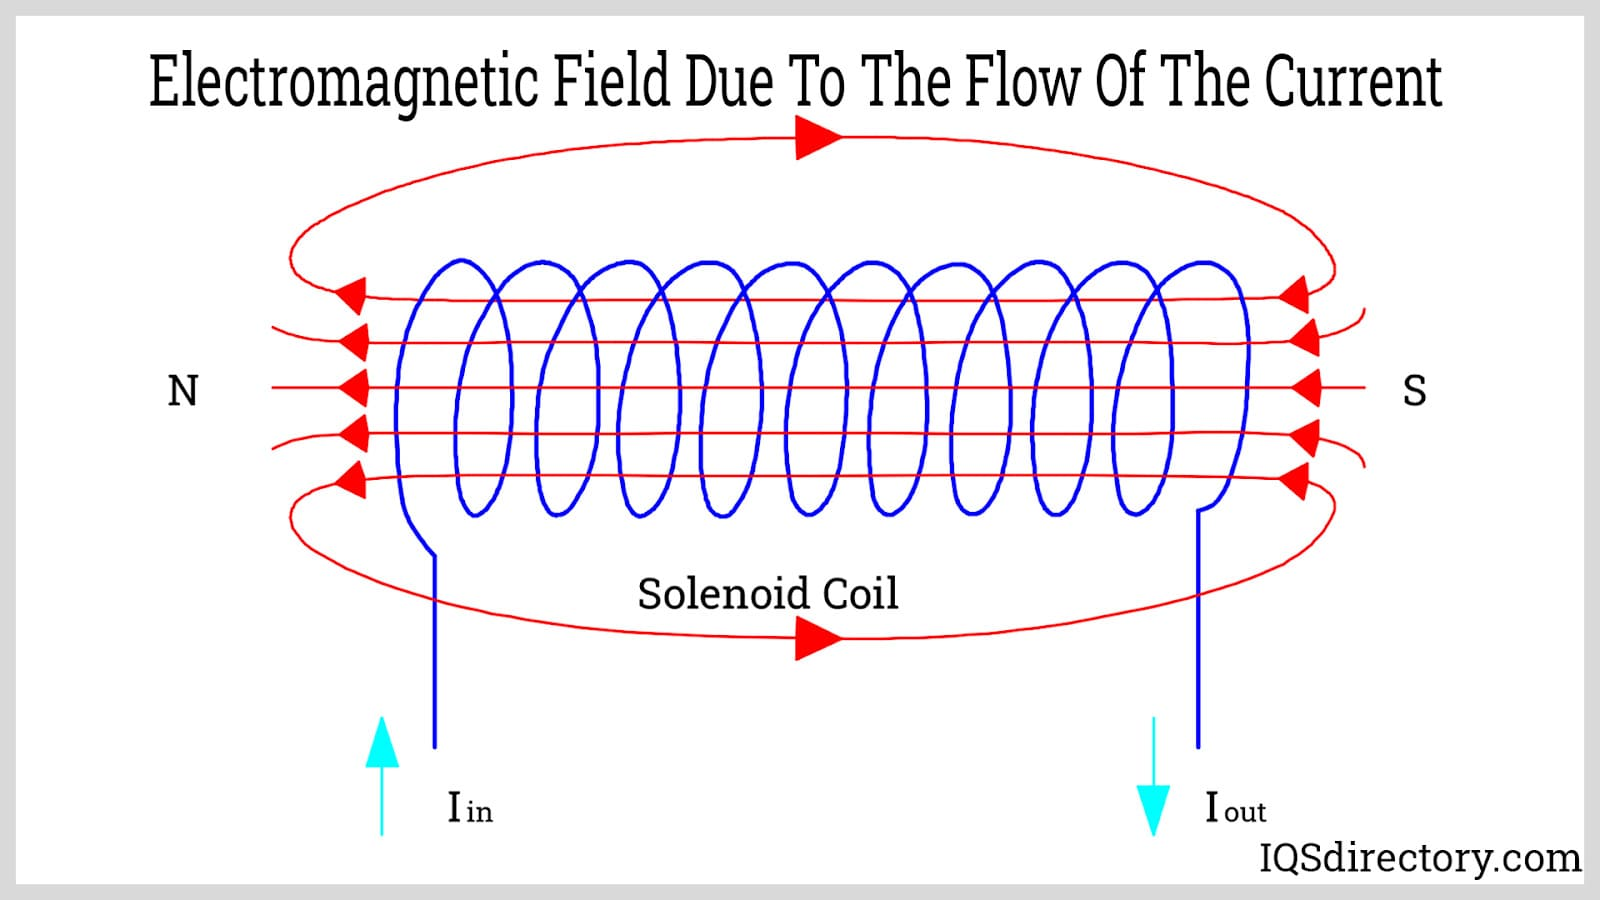
\includegraphics[width=15cm]{solenoid.jpg}
    \centering
    \caption{Electromagnetic Field Due to the Flow of the Current in a Solenoid}
    \label{fig:solenoid}
\end{figure}

\textbf{Capacitance} 

\subsection{Wave Properties}





\subsubsection{Resonance}






\section{The Procedure}



\section{Results and Calculations}



\section{Conclusion}



\section{Expansion on the Experiment}




\newpage


%%%%%%%%%%%%%%%%%%%%%%%%%%%%%%%%%%%

\bibliographystyle{IEEEtran}
\bibliography{References}


\newpage

\section*{Appendix}
\addcontentsline{toc}{section}{Appendix}

\subsection*{Raw Data}
\addcontentsline{toc}{subsection}{Raw Data}

\listoffigures


\end{document}